\documentclass[]{standalone}
%\usepackage{mathptmx}
%\renewcommand{\familydefault}{\rmdefault}
\usepackage[T1]{fontenc}
\usepackage[latin9]{inputenc}
\usepackage{siunitx}
\usepackage{array}
\usepackage{amsmath}
\usepackage{ifthen}
\usepackage{pgfplots}
\pgfplotsset{compat=1.14}
\usepackage{titling, graphicx}
\usepackage{tikz}
\usepackage{upgreek}
\usepackage{amsmath,amsthm}
\usepackage{strtikz}
\usetikzlibrary{shapes,arrows.meta,intersections,graphs,graphs.standard}
\usetikzlibrary{bending, math,fit}
\usetikzlibrary{calc,intersections,through,backgrounds,decorations.pathmorphing}
%\usetikzlibrary{fpu}
%\usepackage{pgfmath}


\begin{document}


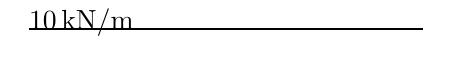
\begin{tikzpicture}
\draw [line width=1](5 cm, 0 cm) -- (0 cm, 0 cm);
\framedistributedspring[startx = 5cm,
starty = 0cm,
endx = 0cm,
endy = 0cm,
number of springs = 5,
space = 0.0cm,
start ratio = 0.02,
end ratio = 0.02,
spring text = $\SI{10}{\kilo\newton/\meter}$,
text shiftx=0pt,
text shifty=0pt,
text location=below,
spring length=0.5cm,
spring prelength ratio=0.2,
spring postlength ratio=0.1,
spring width=0.07cm,
spring segment=0.15cm,
spring scale=1,
spring line thickness=1pt,
spring color=black,
support width=0.3cm,
support depth = 0.1cm,
support line thickness = 1pt,
show support shade=1,
support shade color=gray,]
%$\SI{10}{\kilo\newton/\meter}$
\end{tikzpicture}


\end{document}